% Thesis Chapter 3 — Hardware-aware training taxonomy
% Seeded from manuscript §3 (Methodology) and §5 (Results), with thesis-only ablation depth.
\chapter{Hardware-Aware Training: A Taxonomy of Resampling Cadences, Noise Profiles, and Transfer Guarantees}
\label{chap:hat-taxonomy}

\section{Introduction: HAT as a design space}
\label{sec:hat-design-space}

Hardware-aware training (HAT) is not a single algorithm but a family of training objectives that share one structural feature: they inject a surrogate of the deployment forward-path perturbation into the optimization loop, then back-propagate through a straight-through estimator (STE) so that the digital weight update senses the analog distortion it is supposed to survive. Within that shared skeleton, however, many design choices remain open. How often should the mismatch field be resampled? Should the noise law be uniform, proportional to conductance state, or a mixture of both? And how does the training protocol relate to the formal guarantee one can offer at deployment time?

This chapter treats those choices as axes of a design space rather than as minor implementation details. The thesis perspective differs from the manuscript (manuscript methodology section) in two ways. First, the manuscript presents the canonical fixed-mask, epoch-resampled, and per-batch variants as a short ablation in support of the Ensemble HAT headline; here, each variant receives a formal definition and a distinct transfer-guarantee interpretation. Second, the manuscript discusses proportional-noise retraining primarily as a physical-extension stress test (manuscript NL-HAT stress section); here, it is embedded in a broader taxonomy of noise-profile targeting that clarifies why regime-matched training recovers accuracy while cross-regime deployment collapses.

The chapter is organized as follows. Section~\ref{sec:cadence-definitions} defines the three canonical resampling cadences and visualizes their structural differences. Section~\ref{sec:frequency-sweep} reports the held-out accuracy sweep that isolates epoch-level resampling as the load-bearing schedule choice. Section~\ref{sec:noise-profile-targeting} maps the proportional-versus-additive noise landscape and explains why ``mixed'' profiles are the realistic default for organic optoelectronic arrays. Section~\ref{sec:literature-comparison} situates these choices against DNN+NeuroSim, AIHWKIT, MemTorch, CrossSim, and recent hybrid-mapping literature. Section~\ref{sec:cadence-transfer-guarantee} develops the central thesis insight: the resampling cadence does not merely affect optimization variance; it implicitly defines the distributional family over which the learned classifier is guaranteed to generalize. Section~\ref{sec:summary} summarizes.

\section{Per-batch, per-epoch, and fixed-mask HAT: formal definitions}
\label{sec:cadence-definitions}

All three variants operate on the same hybrid analog--digital inference stack described in the manuscript (manuscript hybrid-deployment section): dense linear operators execute on differential-pair crossbars, control-heavy operators remain digital, and the analog weight is recovered via
\begin{equation}
    \hat{W}_{ij} = s_{\ell}\,G_{\mathrm{eff},ij},
    \qquad
    s_{\ell}=\frac{w_{\max}}{G_{\max}-G_{\min}},
\label{eq:scale-recovery-ch3}
\end{equation}
with layer index $\ell$ omitted for brevity. The effective conductance $G_{\mathrm{eff}}$ is perturbed by a device-to-device (D2D) mismatch field $M$ and by per-forward cycle-to-cycle (C2C) noise $\varepsilon$. The D2D field is spatially structured and fixed for a given hardware instance; the C2C term is independent and identically distributed (i.i.d.) across forward passes.

\subsection{Fixed-mask HAT}

Under \textbf{fixed-mask HAT}, one D2D realization $M_{0}$ is drawn before training and held constant for all epochs and all mini-batches. The optimization objective is the singleton minimisation of Eq.~(\ref{eq:fixed-mask-ch1}) from Chapter~\ref{chap:hat-instance-overfitting}. This is the protocol used by the canonical V4 experiment ($87.95\pm0.27\,\%$ source-domain accuracy) in the manuscript. It is computationally minimal because the mismatch map is cached, and it corresponds to the intuitive strategy of ``training on the hardware you have.'' Its weakness, which Chapter~\ref{chap:hat-instance-overfitting} explores in depth, is that the learned parameters $\theta_{\mathrm{fix}}^{\star}$ can become coupled to the specific spatial signature of $M_{0}$. When the deployment array presents a different fixed realization $M'\sim p(M)$, the calibration and feature routing learned for $M_{0}$ are no longer valid, and accuracy collapses.

\subsection{Ensemble HAT (per-epoch resampling)}

Under \textbf{Ensemble HAT}, the D2D field is resampled at the start of every training epoch and held constant across all mini-batches within that epoch. The objective is the distributional expectation of Eq.~(\ref{eq:ensemble-hat-ch1}) from Chapter~\ref{chap:hat-instance-overfitting}. Because one fresh map is drawn per epoch, the model sees a sequence $\{M^{(1)},M^{(2)},\dots,M^{(E)}\}$ of structured spatial instances. The expectation is Monte Carlo--estimated with $E$ independent draws, where $E$ is the number of training epochs. Crucially, the mini-batch gradients within an epoch are correlated under the same $M^{(e)}$, so the optimizer has enough stationary steps to adapt its feature extraction to that instance before the instance changes. The manuscript reports that this protocol preserves $86.37\pm1.54\,\%$ accuracy on ten fresh hardware instances, overwhelming the chance-level collapse of fixed-mask HAT (manuscript hardware-transferability section).

\subsection{Per-batch resampling}

Under \textbf{per-batch resampling}, a fresh D2D field is drawn independently for every forward pass. The objective is still an expectation over $p(M)$, but the Monte Carlo estimate uses $B\times E$ independent draws, where $B$ is the number of mini-batches per epoch. Formally,
\begin{equation}
    \theta_{\mathrm{batch}}^{\star}=\arg\min_{\theta}\;\mathbb{E}_{M\sim p(M)}\!\left[\frac{1}{N}\sum_{n=1}^{N}\ell\!\left(f(x_{n};\theta,M),y_{n}\right)\right],
\label{eq:hat-batch}
\end{equation}
with the same functional form as Eq.~(\ref{eq:ensemble-hat-ch1}) but a much higher resampling frequency. The training trajectory is now exposed to a new spatial instance every few hundred samples. Intuitively, this might seem preferable because the model sees ``more diversity''; empirically, it underperforms epoch-level resampling because the optimizer never experiences a stable enough forward path to settle into a basin that is compatible with any single structured instance.

\subsection{Visual comparison of the three regimes}

Figure~\ref{fig:cadence-visual} reuses the manuscript's Ensemble HAT concept figure to anchor the discussion, while Table~\ref{tab:cadence-comparison} summarizes the structural properties.

\begin{figure}[t]
    \centering
    
\includegraphics[width=0.78\linewidth]{../latex_gpt/figures/figS3_ensemble_hat}
    \caption{Conceptual comparison of fixed-mask and epoch-resampled HAT, reused from the manuscript package (Figure~1 of the manuscript). The fixed-mask panel shows one spatial mismatch map persisting across all epochs; the Ensemble HAT panel shows a fresh map per epoch. Per-batch resampling (not shown) would replace the map at every mini-batch boundary.}
    \label{fig:cadence-visual}
\end{figure}

\begin{table}[t]
    \centering
    \caption{Structural comparison of the three canonical HAT cadences.}
    \label{tab:cadence-comparison}
    \small
    \begin{tabular}{lccc}
        \toprule
        \textbf{Property} & \textbf{Fixed-mask} & \textbf{Per-epoch} & \textbf{Per-batch} \\
        \midrule
        Resampling frequency & Never & Every epoch & Every mini-batch \\
        Draws per 100 epochs & 1 & 100 & $100B$ \\
        Gradient correlation time & Full training & One epoch & One mini-batch \\
        Forward-path stability & Maximal & Moderate & Minimal \\
        Fresh-instance guarantee & None & Implicit expectation & Implicit expectation \\
        Wall-clock overhead & Baseline & $\sim$1$\times$ & Slightly higher \\
        \bottomrule
    \end{tabular}
\end{table}

Algorithm~\ref{alg:hat-training} gives the unified training loop for all three HAT cadences.
The only difference among the variants is the D2D resampling condition on line~\ref{line:d2d-sample}:
fixed-mask samples once before training ($\mathit{cadence}=\text{never}$),
Ensemble HAT samples at every epoch boundary ($\mathit{cadence}=\text{epoch}$),
and per-batch samples before every mini-batch ($\mathit{cadence}=\text{batch}$).
This unified formulation removes any ambiguity that might remain in prose descriptions.

\begin{algorithm}[t]
\caption{HAT training loop (unified over the three resampling cadences)}
\label{alg:hat-training}
\begin{algorithmic}[1]
\Require Training data $\mathcal{D}=\{(x_n,y_n)\}_{n=1}^{N}$, initial parameters $\theta^{(0)}$, optimizer $\mathcal{O}$
\Require Resampling strategy $\mathit{cadence} \in \{\text{never}, \text{epoch}, \text{batch}\}$
\Require Device profile $\mathcal{P}$, training epochs $E$, batch size $B$
\Ensure Trained parameters $\theta^{(E)}$
\If{$\mathit{cadence} = \text{never}$}
    \State Sample D2D field $\boldsymbol{\epsilon}_{\text{D2D}} \sim \mathcal{N}(0, \sigma_{\text{D2D}}^{2} \Delta G^{2})$ once \Comment{Fixed-mask}
\EndIf
\For{$e = 1, 2, \dots, E$} \Comment{Training epochs}
    \If{$\mathit{cadence} = \text{epoch}$}
        \State Resample D2D field $\boldsymbol{\epsilon}_{\text{D2D}} \sim \mathcal{N}(0, \sigma_{\text{D2D}}^{2} \Delta G^{2})$ \Comment{Ensemble HAT} \label{line:d2d-sample}
    \EndIf
    \For{each mini-batch $\mathcal{B} \subset \mathcal{D}$}
        \If{$\mathit{cadence} = \text{batch}$}
            \State Resample D2D field $\boldsymbol{\epsilon}_{\text{D2D}} \sim \mathcal{N}(0, \sigma_{\text{D2D}}^{2} \Delta G^{2})$ \Comment{Per-batch}
        \EndIf
        \State $\mathcal{L} \gets \frac{1}{|\mathcal{B}|} \sum_{(x,y) \in \mathcal{B}} \ell\bigl(f(x; \theta^{(e)}, \boldsymbol{\epsilon}_{\text{D2D}}, \mathcal{P}), y\bigr)$
        \State Compute $\nabla_{\theta} \mathcal{L}$ via STE back-propagation
        \State $\theta^{(e)} \gets \mathcal{O}.\text{step}(\theta^{(e)}, \nabla_{\theta} \mathcal{L})$
    \EndFor
\EndFor
\State \Return $\theta^{(E)}$
\end{algorithmic}
\end{algorithm}

The distinction between per-epoch and per-batch is subtle but decisive. Per-epoch resampling creates a block-stationary optimization landscape: within each block, the gradient field is consistent, and the optimizer can descend; across blocks, the landscape shifts, forcing the solution toward a shared basin. Per-batch resampling creates a fully non-stationary landscape in which every gradient step sees a different spatial structure. The empirical result, developed in the next section, is that the block-stationary regime yields the best fresh-instance accuracy.

\section{Ensemble frequency sweep: the cadence ablation}
\label{sec:frequency-sweep}

The manuscript notes, in manuscript NL-HAT stress section, that an exploratory single-run training ablation supports the choice of epoch-level resampling. This section unpacks that ablation and places it in the thesis design-space framework.

\subsection{Experimental protocol}

All ablation checkpoints were trained under the canonical Tiny-ViT V4 recipe: AdamW with learning rate $5\times10^{-4}$, weight decay $0.05$, cosine annealing over 100 epochs (the ablation scan used a shortened 50-epoch schedule), batch size 64, and 4-bit differential conductance mapping. The only manipulated variable was the D2D resampling cadence. Three conditions were compared:

\begin{itemize}[leftmargin=1.4em]
    \item \textbf{Fixed-mask control:} One D2D realization drawn at initialization and frozen.
    \item \textbf{Per-epoch (Ensemble HAT):} One fresh D2D realization at the start of each epoch.
    \item \textbf{Per-batch control:} One fresh D2D realization for every forward pass during training.
\end{itemize}

After training, each checkpoint was evaluated on a held-out validation split that was not used for early stopping. The reported numbers are therefore held-out accuracies from a single-run scan, not the full ten-instance fresh-instance protocol reported for the paper-locked Ensemble HAT baseline.

\subsection{Results}

The exploratory scan yielded the following held-out accuracies under the 50-epoch short-run schedule:
\begin{itemize}[leftmargin=1.4em]
    \item Epoch-level resampling (Ensemble HAT): \textbf{88.41\,\%}
    \item Fixed-mask training: \textbf{87.18\,\%}
    \item Per-batch resampling: \textbf{86.16\,\%}
\end{itemize}

These numbers are not directly comparable to the paper-locked $86.37\pm1.54\,\%$ fresh-instance mean because they come from a shorter training run and a held-out validation split rather than the full ten-instance Monte Carlo protocol. Their importance is relative, not absolute: epoch-level resampling outperforms both fixed-mask and per-batch alternatives even under a weakened training budget. Figure~\ref{fig:fresh-instance-ablation} reproduces the manuscript supplementary panel that visualizes this comparison.

\begin{figure}[t]
    \centering
    
\includegraphics[width=0.96\textwidth]{../latex_gpt/figures/fig_fresh_instance_ablation}
    \caption{Fresh-instance robustness and D2D-resampling cadence ablation, reproduced from the manuscript supplementary package (Supplementary Figure~S4). \textbf{Left:} standard HAT collapses to chance on every fresh array, whereas Ensemble HAT preserves robust accuracy. \textbf{Right:} held-out accuracy under different resampling cadences in a 50-epoch scan. Epoch-level resampling reaches 88.41\,\%, exceeding fixed-mask (87.18\,\%) and per-batch (86.16\,\%) controls.}
    \label{fig:fresh-instance-ablation}
\end{figure}

\subsection{Interpretation: why epoch-level resampling wins}

The result is initially surprising because per-batch resampling exposes the model to more D2D diversity and might therefore be expected to produce a more invariant solution. The fact that it underperforms suggests that diversity alone is not the objective; rather, the optimizer needs sufficient time under a single structured instance to learn features that are compatible with that instance, and then enough instances to generalize across the distribution.

Fixed-mask training, by contrast, has unlimited time under one instance and therefore reaches high source-domain accuracy, but it lacks the distributional breadth needed for transfer. Epoch-level resampling sits at a sweet spot: each epoch provides enough stability for the optimizer to make progress, while the sequence of epochs provides enough distributional breadth to prevent instance-specific overfitting.

This interpretation is reinforced by the spatial-versus-i.i.d. ablation discussed in the supplementary package. When the D2D field is replaced by independent per-layer i.i.d. noise drawn every epoch, fresh-instance accuracy drops to approximately 75\,\%; when it is drawn every batch, it drops further to approximately 70\,\%. The structured spatial correlation of the true D2D field, combined with the block-stationary exposure schedule, is the load-bearing ingredient.

\section{Noise-profile targeting: proportional versus additive versus mixed}
\label{sec:noise-profile-targeting}

The cadence discussion assumes a specific noise law: the canonical uniform-noise model in which D2D and C2C perturbations are Gaussian draws scaled by the full conductance window. Real devices, however, often exhibit state-dependent variance. This section extends the taxonomy to the noise-profile axis.

\subsection{Uniform (additive) noise}

Under the \textbf{uniform-noise} regime, the standard deviation of the conductance perturbation is a fixed fraction of the dynamic range:
\begin{equation}
    \sigma_{\mathrm{D2D}} = \alpha\,(G_{\max}-G_{\min}), \qquad \sigma_{\mathrm{C2C}} = \beta\,(G_{\max}-G_{\min}).
\end{equation}
The canonical profile uses $\alpha=10\,\%$ and $\beta=5\,\%$. Because the noise is referenced to the global window, small-conductance devices experience the same absolute perturbation as large-conductance devices. Under the scale-recovery law of Eq.~\ref{eq:scale-recovery-ch3}, many of these perturbations fall below the half-step of the recovered weight grid and are therefore masked. This ``scale-masking'' effect is responsible for the high zero-noise hybrid control accuracy (97.39\,\%) and the relatively mild degradation under canonical uniform noise.

\subsection{Proportional (state-dependent) noise}

Under the \textbf{proportional-noise} regime, the standard deviation scales with the instantaneous conductance magnitude:
\begin{equation}
    \sigma_{\mathrm{D2D}}(G) = \alpha\,|G|, \qquad \sigma_{\mathrm{C2C}}(G) = \beta\,|G|.
\end{equation}
High-conductance states therefore experience larger absolute perturbations than low-conductance states. The scale-masking protection breaks down because the perturbation grows with the signal itself: large weights, which dominate the network's output, also receive the largest relative noise. When a model trained under uniform noise is evaluated under proportional noise, accuracy collapses to 10.00\,\% for Tiny-ViT V4, indicating that the uniform model overestimates intrinsic robustness.

Crucially, proportional noise is not merely a stress test; it is the physically expected regime for ohmic conductance channels and for several organic device families in which conductance fluctuations track the mean. The manuscript therefore treats proportional-noise HAT as a regime-matched training experiment rather than an adversarial perturbation.

\subsection{Mixed profiles}

A \textbf{mixed} noise profile superimposes a floor (uniform) component and a state-dependent (proportional) component:
\begin{equation}
    \sigma(G) = \sigma_{0} + \kappa\,|G|.
\end{equation}
This form captures the empirical reality that real arrays exhibit both a baseline fabrication spread (uniform) and a state-dependent read or programming fluctuation (proportional). The framework supports mixed profiles through the JavaScript Object Notation (JSON) device-profile interface (manuscript profile-interface section), although the canonical paper experiments use pure uniform or pure proportional modes for interpretability.

\subsection{Regime-matched training and cross-regime collapse}

The manuscript reports that proportional-noise HAT recovers Tiny-ViT to $97.37\pm0.05\,\%$ when training and evaluation are both conducted under the proportional law. This demonstrates that the proportional regime is learnable. However, the same checkpoint transfers poorly back to uniform-noise evaluation, and a uniform-noise checkpoint collapses under proportional evaluation. The takeaway is that HAT robustness is \emph{distribution-specific}: the training objective must match the deployment noise law, and there is no free cross-regime generalization.

Table~\ref{tab:noise-regime-matrix} summarizes the cross-regime behavior for Tiny-ViT. The diagonal entries (matched training and evaluation) are high; the off-diagonal entries (mismatched) are low. This matrix is a central tool for deciding which noise model to adopt as the canonical profile: if the physical device is believed to operate in the proportional regime, then uniform-noise HAT is an optimistic fiction; conversely, if the device is primarily uniform, proportional-noise training is unnecessarily pessimistic.

\begin{table}[t]
    \centering
    \caption{Cross-regime accuracy matrix for Tiny-ViT under uniform and proportional noise. Diagonal entries are matched-regime results; off-diagonal entries show cross-regime collapse.}
    \label{tab:noise-regime-matrix}
    \small
    \begin{tabular}{lcc}
        \toprule
        & \textbf{Eval: Uniform} & \textbf{Eval: Proportional} \\
        \midrule
        Train: Uniform (V4) & $\sim$91\,\% & 10.00\,\% \\
        Train: Proportional & $\sim$10.38\,\% & 97.37\,\% \\
        \bottomrule
    \end{tabular}
\end{table}

\section{Related work}
\label{sec:literature-comparison}

The design-space axes developed above are not unique to this thesis. DNN+NeuroSim established the hierarchical device-to-system evaluation template for CIM \citep{peng2020dnnneurosim}; AIHWKIT provides a PyTorch-integrated toolkit with per-batch PCM/ReRAM noise injection \citep{rasch2021aihwkit}; MemTorch embeds memristive non-idealities natively in PyTorch but focuses on inference-time fault injection rather than training-time resampling cadences \citep{lammie2022memtorch}; and CrossSim offers GPU-accelerated lookup-table-based training with parasitic resistance and ADC models \citep{crosssim2026}. None of these frameworks, however, exposes structured D2D mismatch resampling as a first-class training hyperparameter. The hybrid analog--digital mapping used here---linear projections on crossbars, attention and normalization in digital---is independently adopted by recent heterogeneous accelerators such as HARDSEA \citep{lin2024hardsea}, confirming that the partition is a broadly sensible architectural response rather than a simulator artifact. Ensemble HAT is conceptually related to domain randomization in sim-to-real robotics \citep{tobin2017domain}, but the latter randomizes i.i.d. environmental parameters, whereas D2D mismatch is a spatially correlated fixed field; the thesis ablation showing that i.i.d. per-epoch noise drops fresh-instance accuracy to $\sim$75\,\% (versus 86.37\,\% for structured resampling) confirms that correlation-aware augmentation is the load-bearing ingredient.

\section{Thesis insight: resampling cadence as an implicit transfer guarantee}
\label{sec:cadence-transfer-guarantee}

The empirical results of Sections~\ref{sec:frequency-sweep} and \ref{sec:noise-profile-targeting} can be unified under a single theoretical observation: the resampling cadence implicitly defines the distributional family over which the learned classifier is guaranteed to generalize.

\subsection{Fixed-mask HAT: singleton guarantee}

Fixed-mask HAT is a singleton minimisation: it trains on a single D2D draw $M_{0}$ and minimises the empirical risk conditioned on that draw. The guarantee it offers is trivial: the model is guaranteed to perform well on $M_{0}$ itself, and on nothing else. Formally, if $\mathcal{R}(\theta,M)$ denotes the risk under mismatch map $M$, then fixed-mask HAT minimizes $\mathcal{R}(\theta,M_{0})$ and provides no bound on $\mathcal{R}(\theta,M')$ for $M'\neq M_{0}$. The 10.00\,\% fresh-instance collapse is the empirical signature of this absence of guarantee.

\subsection{Per-batch HAT: product-distribution guarantee}

Per-batch resampling solves Eq.~\ref{eq:hat-batch} with $B\times E$ independent draws. The optimizer therefore sees a product distribution $p(M)^{\otimes(B\times E)}$ over mismatch maps, but each gradient step is computed under a single independent draw. The resulting solution minimizes the expected risk under the marginal distribution $p(M)$, but the high variance of the gradient estimates prevents the optimizer from finding a basin that is simultaneously compatible with any single structured instance. The empirical result---86.16\,\% held-out accuracy, lower than per-epoch---suggests that the product-diversity guarantee is too weak: the model learns to survive average noise, but not any specific realization.

\subsection{Per-epoch HAT: block-stationary guarantee}

Per-epoch resampling generalises this to $E$ block-stationary draws. Within each block, the optimizer descends under a fixed $M^{(e)}$; across blocks, it seeks a shared basin. The implicit guarantee is stronger than the product-distribution guarantee because the optimizer must find a parameter vector that is not merely good in expectation, but good for at least one full epoch of descent under each of $E$ independent realizations. The empirical result---88.41\,\% held-out accuracy, and $86.37\pm1.54\,\%$ on fresh instances---suggests that this block-stationary requirement is sufficient to force the model into a basin that generalizes across the deployment distribution.

\subsection{Noise-profile matching as a distributional alignment condition}

The same logic extends to noise profiles. A model trained under uniform noise minimizes risk under the uniform noise distribution $p_{\mathrm{uni}}(M)$; a model trained under proportional noise minimizes risk under $p_{\mathrm{prop}}(M)$. Because $p_{\mathrm{uni}}$ and $p_{\mathrm{prop}}$ are mutually singular in the large-perturbation tail, a classifier that is optimal under one is not guaranteed to be even admissible under the other. The 10.00\,\% cross-regime collapse is the empirical signature of this distributional misalignment.

The practical consequence is that the choice of noise profile is not a secondary modeling detail; it is a distributional prior that must be matched to the physical device. A simulator that defaults to uniform noise will overestimate deployment accuracy for devices that follow a proportional law. The profile-driven substitution interface (manuscript profile-interface section) is therefore not merely a convenience feature; it is the mechanism by which the training objective is aligned with the physical deployment distribution.

\subsection{Summary: the cadence--profile design plane}

Figure~\ref{fig:design-plane} sketches the two-dimensional design plane formed by the cadence axis (fixed / epoch / batch) and the noise-profile axis (uniform / proportional / mixed). The thesis experiments occupy specific points on this plane:

\begin{itemize}[leftmargin=1.4em]
    \item \textbf{Manuscript canonical V4:} fixed-mask, uniform noise.
    \item \textbf{Manuscript Ensemble HAT:} per-epoch, uniform noise.
    \item \textbf{Manuscript proportional-noise HAT:} per-epoch, proportional noise.
    \item \textbf{This chapter's ablation:} per-epoch versus fixed versus per-batch, uniform noise.
\end{itemize}

The design plane is a tool for future work: if a new device profile suggests, for example, that spatial correlation decays over shorter length scales, one can move to a finer cadence (per-epoch with multiple maps per epoch) or to a coarser one (fixed-mask with a worst-case map). The framework's modularity makes such movements possible without code changes.

\begin{figure}[t]
    \centering
    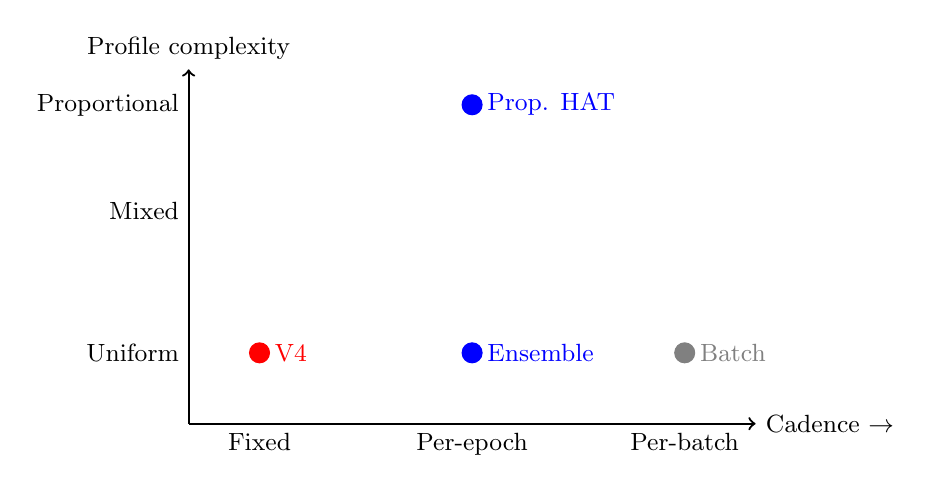
\begin{tikzpicture}[scale=0.9, every node/.style={font=\small}]
        \draw[->,thick] (0,0) -- (8,0) node[right] {Cadence $\rightarrow$};
        \draw[->,thick] (0,0) -- (0,5) node[above] {Profile complexity};
        \node[below] at (1,0) {Fixed};
        \node[below] at (4,0) {Per-epoch};
        \node[below] at (7,0) {Per-batch};
        \node[left] at (0,1) {Uniform};
        \node[left] at (0,3) {Mixed};
        \node[left] at (0,4.5) {Proportional};
        \filldraw[red] (1,1) circle (4pt) node[right, xshift=2pt] {V4};
        \filldraw[blue] (4,1) circle (4pt) node[right, xshift=2pt] {Ensemble};
        \filldraw[blue] (4,4.5) circle (4pt) node[right, xshift=2pt] {Prop. HAT};
        \filldraw[gray] (7,1) circle (4pt) node[right, xshift=2pt] {Batch};
    \end{tikzpicture}
    \caption{Simplified design plane for HAT protocols. The horizontal axis moves from fixed-mask (no resampling) to per-batch (maximal resampling). The vertical axis moves from uniform additive noise to proportional state-dependent noise. Thesis experiments occupy the labeled points.}
    \label{fig:design-plane}
\end{figure}

\section{Summary}
\label{sec:summary}

This chapter has treated hardware-aware training as a design space with two primary axes: resampling cadence and noise-profile targeting.

On the \textbf{cadence axis}, three canonical protocols were defined: fixed-mask HAT, per-epoch Ensemble HAT, and per-batch resampling (Eq.~\ref{eq:hat-batch}). An exploratory 50-epoch ablation showed that epoch-level resampling reaches 88.41\,\% held-out accuracy, outperforming both fixed-mask (87.18\,\%) and per-batch (86.16\,\%) controls. The interpretation is that block-stationary exposure---one structured instance per epoch---provides enough forward-path stability for the optimizer to descend, while the sequence of epochs provides enough distributional breadth to prevent instance-specific overfitting.

On the \textbf{noise-profile axis}, uniform (additive), proportional (state-dependent), and mixed noise laws were compared. Proportional noise destroys the scale-masking protection that makes uniform-noise models appear robust, and regime-matched training is required for recovery. A model trained under uniform noise collapses to 10.00\,\% under proportional evaluation, and vice versa, demonstrating that HAT robustness is distribution-specific.

Against the \textbf{literature}, the framework was positioned relative to DNN+NeuroSim (hierarchical benchmarking), AIHWKIT (per-batch stochastic variation), MemTorch (PyTorch-native embedding), CrossSim (lookup-table training), and the HARDSEA hybrid-mapping architecture of Lin~\emph{et al.}~(including Q.~Qin). The thesis adds value not by outperforming these mature tools on inorganic benchmarks, but by exposing how the same hybrid mapping behaves under organic-specific noise laws and under different HAT cadences.

The central \textbf{thesis insight} is that the resampling cadence implicitly defines the transfer guarantee. Fixed-mask HAT offers a singleton guarantee (valid only on the training instance), per-batch HAT offers a product-distribution guarantee that is too weak for structured spatial mismatch, and per-epoch HAT offers a block-stationary guarantee that empirically generalizes to fresh hardware instances. The taxonomy reveals symptoms, but symptoms are not diagnoses; the next chapter names the diseases.  Physical-realism extensions in Chapter~\ref{chap:physical-realism} validate that the block-stationary guarantee survives correlated D2D and retention drift.
